\documentclass[11pt,a4paper]{article}
\usepackage[hyperref]{emnlp2018}
\usepackage{times}
\usepackage{latexsym}
\usepackage{url}

\usepackage{amsmath}
\usepackage{amssymb}
\usepackage{bm}
\usepackage{booktabs}
\usepackage{caption}
\usepackage{CJKutf8}
\usepackage[inline,shortlabels]{enumitem}
\usepackage[T1]{fontenc}
\usepackage{footnote}
\usepackage{graphicx}
\usepackage[utf8]{inputenc}
\usepackage{multirow}
\usepackage{pifont}
\usepackage{subcaption}
\usepackage{tikz}
\usepackage{verbatim}
\usepackage{wrapfig}
\usetikzlibrary{fit,positioning}
\makesavenoteenv{table}
\makesavenoteenv{tabular}

\aclfinalcopy % Uncomment this line for the final submission
%\def\aclpaperid{***} % Enter the acl Paper ID here

%\setlength\titlebox{5cm}

%\renewcommand{\baselinestretch}{1.04}

\newcommand{\ensuretext}[1]{#1}
\newcommand{\mycomment}[3]{\ensuretext{\textcolor{#3}{[#1 #2]}}}
\newcommand{\ammarker}{\ensuretext{\textcolor{blue}{\ensuremath{^{\textsc{A}}_{\textsc{M}}}}}}
\newcommand{\am}[1]{\mycomment{\ammarker}{#1}{blue}}
\newcommand{\cjdmarker}{\ensuretext{\textcolor{red}{\ensuremath{^{\textsc{C}}_{\textsc{D}}}}}}
\newcommand{\cjd}[1]{\mycomment{\cjdmarker}{#1}{red}}
\newcommand{\gnmarker}{\ensuretext{\textcolor{green}{\ensuremath{^{\textsc{G}}_{\textsc{N}}}}}}
\newcommand{\gn}[1]{\mycomment{\gnmarker}{#1}{green}}
\newcommand{\ignore}[1]{}
\newcommand{\cmark}{\ding{51}}%
\newcommand{\xmark}{\ding{55}}%
\newcommand{\pluseq}{\mathrel{+}=}
\DeclareMathOperator*{\argmax}{arg\,max}
\DeclareMathOperator*{\argmin}{arg\,min}

\title{Monte-Carlo Tree Search for Machine Translation Inference}

\author{Austin Matthews \and Graham Neubig \\
  Language Technologies Institute \\
  Carnegie Mellon University \\
  {\tt \{austinma,gneubig\}@cs.cmu.edu} \\\And
  Chris Dyer \\
  DeepMind \\
  {\tt cdyer@google.com} \\}
\date{}

\hypersetup{draft}
\begin{document}
\maketitle

\begin{abstract}
Many NLP algorithms rely on greedy or beam search to find a globally optimal
hypothesis in the forest of possibilities produced by a locally normalized
sequential model. In this work we show that Monte-Carlo Tree Search (MCTS)
offers a compelling replacement that allows us to search using a broader class
of models, including non-normalized moels. This flexibility admits previously
intractable approaches that can yield problem-specific improvements.
While most of the techniques discussed are abstract and applicable to many NLP
tasks, we demonstrate improvements on a machine translation task, resulting in
improved BLEU score as well as model loss relative to a beam search baseline.
\end{abstract}

\section{Introduction}
\label{sec:intro}
Many tasks in natural language processing, such as parsing, language modelling,
speech recognition, and machine translation, lend themselves to sequential
algorithms. Such algorithms typically begin in some initial \emph{state} (e.g.
an empty string, or a bare \textsc{root} node) and use an locally normalized
model to choose its next \emph{action} (e.g. emit word $w$, or take parsing
transition $t$). To get a full transcript, parse tree, or translation then
requires a non-trivial search to find a single hypothesis that globally
maximizes a scoring function. In the NLP world to date the most popular search
algorithm has been \emph{beam search}
\cite[inter alia]{koehn2004pharaoh,bahdanau2014neural,vinyals2015grammar,
vaswani2017attention}.

Monte-Carlo Tree Search (MCTS), on the other hand, is a search algorithm most
commonly used by game-playing programs. In particularly excels for games where
\begin{enumerate*}[(a)]
\item evaluating a non-terminal position is difficult,
\item the branching factor is large, and 
\item actions taken now show complex interactions with later actions.
\end{enumerate*}
MCTS has enjoyed particularly large
success in the Go AI community \cite{abramson1987model, brugmann1993monte,
silver2017mastering}.

Many NLP tasks, such as machine translation, can be seen as single player games in which
the single player attempts to search for a series of actions that maximizes a final score.
Furthermore, such tasks exhibit all three of the above properties, and thus lend themselves
nicely to MCTS-based solutions.

\section{Beam Search}
\label{sec:beam_search}
The beam search algorithm (with beam width $k$) begins in its initial state
$s_0$ and queries its model for the $k$ actions that seem the most promising
locally. It then creates new nodes in its search tree for each of these $k$
children and again queries its model for the $k$ most promising actions from
each child state. Of the $k^2$ frontier nodes now in the search tree, the top $k$
are kept and all others are discarded and searched no further. The algorithm
continues this process recursively; at each step it has (up to) $k$ states to
expand, gets the locally best $k$ actions for each, and then keeps the top $k$
of the resulting $k^2$ candidate nodes.

While beam search is a strong baseline, and is the most common decoding
algorithm used for generation tasks (e.g. MT, action-based parsing, language
modelling), it is not without drawbacks.

First, beam search constrains each node in its search graph to have the same
fan out. The algorithm searches $k$ child nodes no matter what, including from
nodes where the neural network is very confident in what the next word will be
(i.e. where the distribution over potential next actions has very low entropy).
Conversely, it can \emph{only} search $k$ child nodes, even if the entropy over
children is very high.

Second, it relies on a local scoring function, where the underlying model takes
a node and predicts, given only its previously-generated context, the next word
in the output sequence. This means that beam search can never leverage
information about what occurs later in the sentence, or about the global
quality of its output. In the context of neural machine translation, this leads
to the output of beam search being very fluent, but often unfaithful to the
source sentence. Furthermore, output tends to be shorter than desired, leading
to depressed BLEU scores \cite{koehn2017six}.

\section{Monte-Carlo Tree Search}
\label{sec:mcts}
Monte-Carlo Tree Search also begins from an initial state $s_0$ and intelligently
samples promising paths through the search tree. With each sample it gains further
statistical insight into which action sequences are good and bad, allowing it
to gradually hone in on the optimum. In theory MCTS
does not even need a local model to choose its next action (instead choosing
uniformly at random), though in practice one is typically used as a \emph{prior}
to guide the algorithm towards good parts of
the search space, speeding up convergence dramatically.
 In the first subsection below (\S \ref{sec:mcts_alg})
we outline how the MCTS algorithm works.
In the second, we discuss the design how the nature of the MCTS algorithm
admits additional flexibility in how hypotheses are scored and examine
some choices of good scoring functions.

\subsection{The MCTS Algorithm}
\label{sec:mcts_alg}
The MCTS algorithm consists of four steps: selection, expansion, simulation,
and backpropagation \cite{chaslot2008progressive}. This sequence of four steps
is repeated until the user is satisfied with performance or has exhausted his or
her patience. Each node $n$ in the search tree stores three pieces of
information, all floats:
\begin{enumerate*}[(1)]
\item the sum (``total'') of the scores resulting in simulations descended from this node, denoted $n_t$
\item the number of times the node has been visited, denoted $n_n$, and
\item the prior probability of this node given its parent's state, denoted $n_p$
\end{enumerate*}.

\paragraph{Selection}
Starting from the root node the algorithm recursively selects the child
$\hat{c}$ that maximizes $\text{PUCT}(c)$, defined below, until it reaches a
node with visit count 0.

$\text{PUCT}(c) = \frac{c_t}{c_n} + k_{\text{puct}} \cdot c_p \cdot
\frac{\sqrt{n_n}}{c_n + 1}$, where $k_{\text{puct}}$ is a user-defined
exploration constant. The first term is the average value achieved by all
simulations that pass through this child node. The second term is proportional
to the a priori probability of a child node and inversely proportional to the
number of times we have already visited it, thus encouraging the model to visit
nodes that seem good a priori but have been visited relatively few times.

Special care must be taken to handle the case where $c_n = 0$. Many approaches
are feasible, the simplest being to let $\text{PUCT}(c) = \infty$ when $c_n =
0$, leading to exploring all possible next states at least once before
repetition. More advanced approaches (e.g. \newcite{gelly2007combining}) seek
to approximate $\lim\limits_{N \to \infty} \text{PUCT}(c)$ using the
information available, which includes the parent and sibling nodes' statistics,
as well as the prior probabilities of the unvisited node and its siblings. We
choose to approximate $\text{Value}(c) \approx \text{Value}{p} + (c_p -
\hat{c}_p)$, where $\hat{c} = \argmax_{c} c_p$. The intuition behind this
choice is that a priori we believe that the value of the highest scoring child
($\hat{c}$) should be similar to the value of its parent and that other nodes
will likely lag behind the score of $\hat{c}$ by an amount consistent with the
difference in their values according to the model.

\paragraph{Expansion}
Expand the current node (which has visit count 0 since we just finished the
selection step), by running the neural network to get prior probabilities and
then creating and initializing all possible child nodes.

\paragraph{Simulation}
From the current node randomly sample words (according to the NN's distribution
at each step) until reaching an $\textsc{</s>}$. Evaluate the resulting
sentence to get some score $s$. In the MCTS literature each simulation is
called a \emph{rollout}.

\paragraph{Backpropagation}
Update statistics for each node $n$ visited during the tree exploration phase,
from the root down to the node from which the simulation started, and update
$n_t \pluseq s$ and $n_n \pluseq 1$.

\subsection{Scoring Function}
\label{sec:mcts_score}
Perhaps the most intriguing feature of the MCTS search algorithm is that only
terminal nodes (which, in our case, represent full sentences ending with
\textsc{</s>}) are ever scored. This opens up many new possibilities for the
scoring function, since it no longer need be decomposible over edges in the
search graph. The most straight forward scoring function is the simple
conditional (log-)probability of the sentence, $p(t|s)$. This is the score that
is optimized by beam search and other search algorithms since it is nicely
edge-decomposable.

The relaxation of the decomposability requirement, however, allows us to use
more interesting (and hopefully more informative) scoring functions. For
example if we have a ``reverse'' NMT system and thus have access to a model of
$p(s|t)$ we might define our scoring function to be $\lambda_0 p(t|s) +
\lambda_1 p(s|t)$ for some choice of $\lambda$s. Furthermore, if we have access
to a language model that gives probabilities $p(t)$, we could add an additional
term $\lambda_2 p(t)$.
Note that unlike traditional MT models, these lambdas are \emph{not} scale-invariant,
due to their interaction with $c_\text{PUCT}$ in the selection step of MCTS.

While one can clearly tune these $\lambda$s as While we choose to tune these
$\lambda$s we note here one particularly interesting possible choice. If one
lets $\lambda_0 = 0$, $\lambda_1 = 1$ and $\lambda_2 = 1$, then this gives us
the neural equivalent of the classic noisy channel model of machine
translation. As we will see in \S\ref{sec:experiments}, such a system performs
quite well, only slightly behind our best tuned set of weights.

\section{Experiments}
\label{sec:experiments}
Though our MCTS-based approach to decoding is generally applicable to any
problem based on a sequence of actions, in this work we use the problem
of machine translation to demonstrate its effectiveness.

\subsection{Data Set}
\begin{table}
\centering
\begin{tabular}{r r c c}
\toprule
& & Sents & Words \\
\midrule
 & Train & 44K & 336K \\
& Dev & 1006 & 7627 \\
& Test & 506 & 3906 \\
\bottomrule
\end{tabular}
\caption{Details of our data set.}
\label{tab:data_sets}
\end{table}

We experiment on the Chinese--English Basic Travel Expression Corpus (BTEC)
\am{how do we cite this?},
a relatively small corpus consisting of short travel-related sentences.
The vocabularies used have 3429 Chinese types and 3115 English types.

\subsection{Baselines}
In all experiments we use a standard LSTM-based attention model
\cite{bahdanau2014neural} implemented in the xnmt toolkit
\cite{neubig2018xnmt}. All of our models use 128-dimensional word embeddings
and 512-dimensional LSTM states. We train using the Adam optimizer
\cite{kingma2014adam} with a learning rate of 0.001 for 20 epochs, use dropout
\cite{srivastava2014dropout} with $p=0.3$, and use minibatches with an average
size of 32 sentences. Any other parameters use xnmt's default values. We use
beam search decoding as our baseline and perform a hyperparameter search for
the optimal value of $k$.

\subsection{MCTS Hyperparameter Tuning}
For our MCTS approach we have to tune $c_\text{puct}$ and the $\lambda$s. We
begin by using only the forward model (i.e. $\lambda_0=1$, $\lambda_1=0$,
$\lambda_2=0$), keeping the number of visits per sentence constant, and varying
$c_\text{puct}$ \footnote{See Table~\ref{tab:btec_mcts_cpuct} in the appendix
for results}.

With an optimal value of $c_\text{puct}$ chosen we can now compare MCTS (using
only the forward model) to our beam search baseline.

Finally, we run MCTS using three models: $p(\text{en}\mid\text{zh})$,
$p(\text{zh}\mid\text{en})$, and $p(\text{en})$. We run a grid search over
quick experiments using 200 rollouts over an 8x8x8 grid of possible values of
the three $\lambda$ parameters and take the setting that maximizes
BLEU\footnote{See Figure \ref{fig:grid_search} in the appendix for full
results}. To ensure a fair comparison to beam search, we take the $k$-best list
produced by beam search, compute each hypothesis's score under each of the
three model, and choose the hypothesis with the best score, using the set of
weights found above.

\section{Results}
\label{sec:results}
Table~\ref{tab:btec_bs_results} shows the results of beam search, with varying
settings of $k$, peaking at $k=50$ with 46.76 BLEU.
Table~\ref{tab:btec_mcts_rollouts} shows the results of running single-model
MCTS with various numbers of simulations per sentence, peaking at 47.08 BLEU
with 1000 rollouts per sentence. Unlike beam search, MCTS seems to continue to
improve translation quality as more time is spent on decoding. It is likely
further (if marginal) gains could be realized by continuing to increase the
number of rollouts per sentence. \am{Easy to test this with n=2000, 5000, or
even 10-2000}.

\begin{table}
\centering
\resizebox{0.8\columnwidth}{!}{%
\begin{subtable}[t]{.45\linewidth}
\flushright
\begin{tabular}{r l l}
\toprule
$k$ & BLEU & Loss \\
\midrule
1 & 42.69 & 0.46 \\
2 & 45.14 & 0.41 \\
5 & 46.42 & \textbf{0.40} \\
10 & 46.65 & \textbf{0.40} \\
20 & 46.53 & \textbf{0.40} \\
50 & \textbf{46.76} & \textbf{0.40} \\
100 & 46.63 & \textbf{0.40} \\
200 & 46.50 & \textbf{0.40} \\
\bottomrule
\end{tabular}
\caption{Results with beam search on our dev set.}
\label{tab:btec_bs_results}
\end{subtable}
\hspace{\fill}
\begin{subtable}[t]{.45\linewidth}
\flushright
\begin{tabular}{r l l}
\toprule
Rollouts & BLEU & Loss \\
\midrule
1 & 42.69 & 0.45 \\ 
2 & 42.69 & 0.45 \\
5 & 42.80 & 0.45 \\
10 & 43.06 & 0.45 \\
20 & 43.69 & 0.44 \\
50 & 45.01 & 0.43 \\
100 & 45.90 & 0.42 \\
200 & 46.71 & \textbf{0.41} \\
500 & 46.68 & \textbf{0.41} \\
1000 & \textbf{47.08} & \textbf{0.41} \\
\bottomrule
\end{tabular}
\caption{Results with MCTS on our dev sets with $c_{\text{puct}}=20$, the best
value found, varying the number of rollouts.}
\label{tab:btec_mcts_rollouts}
\end{subtable}
}
\end{table}

Figure \ref{fig:3models} compares the loss under (rescored) beam search
and three-model MCTS. Beam search achieves a maximum BLEU score of 48.83
and a minimum per-word loss of 3.06. MCTS achieves a maximum BLEU score of
49.51 and a minimum loss of 3.03.

\begin{figure}
\centering
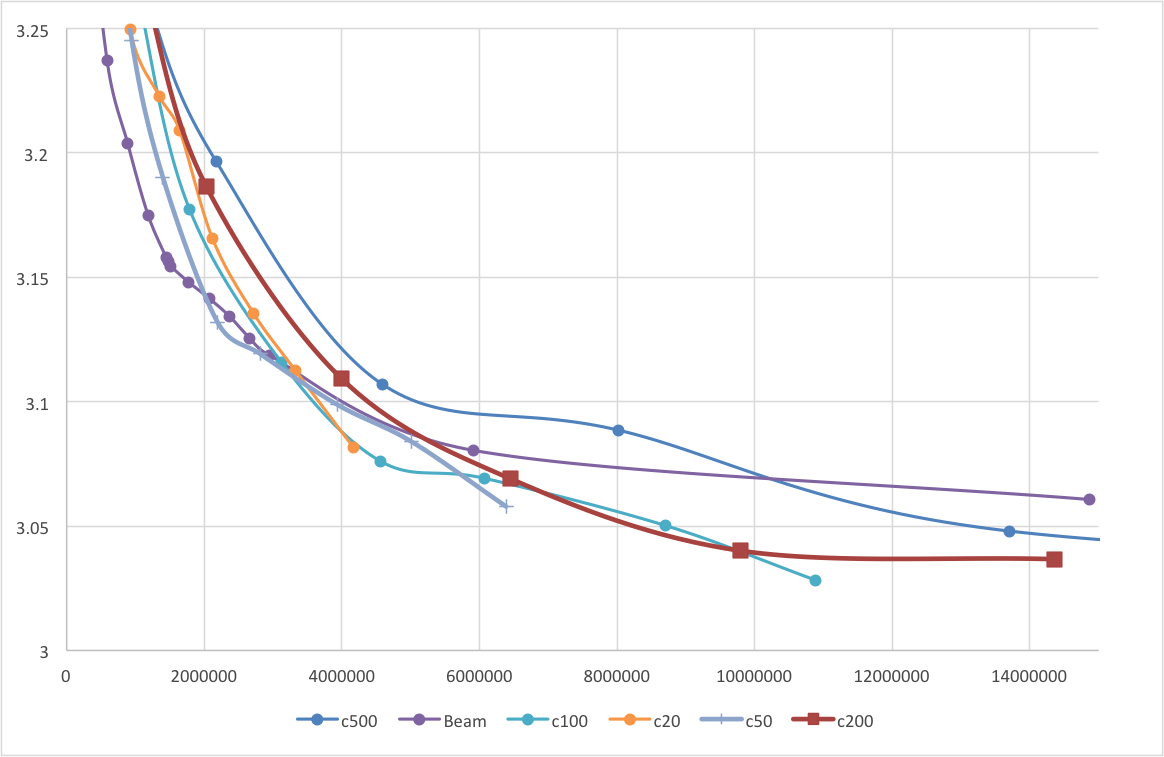
\includegraphics[scale=0.35]{mcts_3models.png}
\caption{Comparison of loss values (y-axis) vs. number of softmaxes (x-axis) using rescored k-best lists
or MCTS using three models.}
\label{fig:3models}
\end{figure}

\section{Analysis}
\label{sec:analysis}

\begin{figure}
\centering
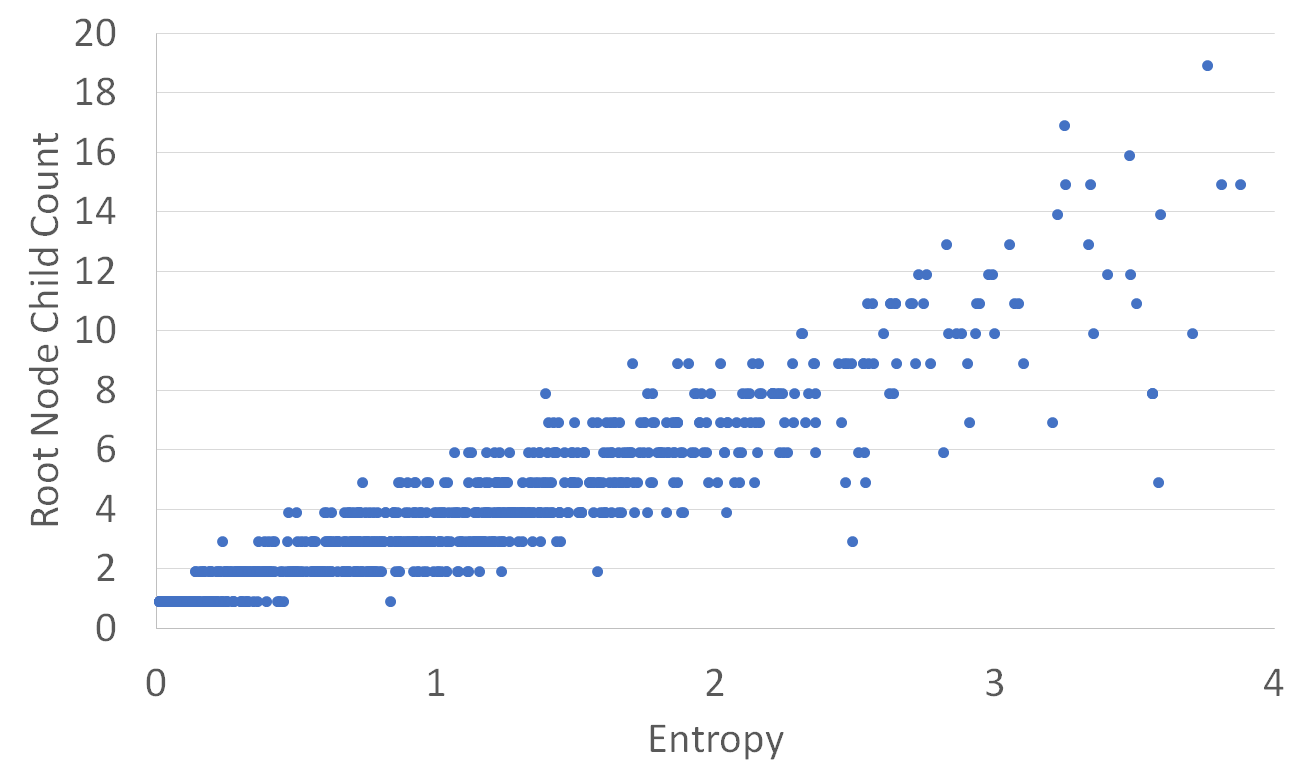
\includegraphics[scale=0.2]{branch_entropy.png}
\caption{Plot of the entropy versus the number of children (fan out) of root
nodes when using single-model MCTS with $c_{\text{puct}}=20$ and 200 rollouts.}
\label{fig:entropy}
\end{figure}

We posit that the improvements from MCTS come from its ability to more
thoroughly explore interesting parts of the search space while ignoring the
less promising parts. To explore this hypothesis we examine how the branching
factor of the MCTS search changes as a function of the entropy of the
distribution output by the neural network. To avoid the effects of varying
number of visits, we limit our analysis to the root nodes of each of the 1006
sentences in our development set. The results are shown in \ref{fig:entropy}.
We can see that our algorithm explores many possible children when a node's
entropy is high and few nodes when the entropy is low. The average number of
children is 3.55 with a standard deviation of 2.78.

\section{Related Work}
\label{sec:related_work}
Other work has addressed the problem of beam search's fixed fan out without
abandoning the beam search paradigm as dramatically as we have.
\newcite{freitag2017beam} examine pruning strategies other than simply keeping
the top $k$ words at each timestep, including keeping everything within a
constant amount (either additively or multiplicatively) from the best
hypothesis.

\newcite{vijayakumar2016diverse} address the limited diversity of beam search's
outputs, a symptom of its inability to capture long-distance interactions
within hypotheses. \newcite{sun2017bidirectional} also address this
insufficiency in beam search, using a bi-directional search model. While their
bidirectional model allows for some propogation of information, but is limited
by their first-order Markov assumption.

The MCTS algorithm was originally developed for playing the game of Go
\cite{coulom2006efficient}, for which there is no known evaluation function,
and which has extremely complex long-distance interactions between moves. It
was quickly extended to simple single player games \cite{schadd2008single},
where it also showed good performance. A few years later
\newcite{maes2012monte} characterized a whole family of MCTS-based methods and
searches for the best variants on a suite of single-player games. Separately
\newcite{baier2012beam} proposed an intriguing hybrid of MCTS and Beam Search
and use it to play one-player games.

More recently \newcite{silver2016mastering} introduced neural priors into MCTS,
bringing Go AI to super-human levels for the first time. Their technique has
since been expanded to many other domains with great success \cite[inter
alia]{silver2017mastering,pinheiro2017geometric,lee2018deep,luckow2018monte}.

\section{Conclusion}
In this work we have applied Monte-Carlo Tree Search to the domain of neural
machine translation.
We have shown that MCTS can compete with beam search and admits exciting new
possibilities for searching with a diverse set of models.
We have demonstrated gains in both BLEU and model score for Chinese--English
machine translation, both in the one-model setting and the three-model setting.

\section*{Acknowledgements}
\label{sec:acknowledgements}
Matthias for help with LMs in xnmt.
Grants?

\bibliography{biblio}
\bibliographystyle{acl_natbib_nourl}

\clearpage

\appendix
\section{Extra Tables and Figures}

\begin{table}
\centering
\begin{tabular}{r l l}
\toprule
$c_{\text{puct}}$ & BLEU & Loss \\
\midrule
0.1 & 40.82 & 0.56 \\
0.2 & 40.57 & 0.55 \\
0.5 & 41.77 & 0.54 \\
1 & 42.46 & 0.52 \\
2 & 42.96 & 0.51 \\
5 & 44.86 & 0.45 \\
10 & 46.07 & 0.42 \\
20 & \textbf{46.71} & \textbf{0.41} \\
50 & 45.22 & 0.42 \\
100 & 44.63 & 0.42 \\
\bottomrule
\end{tabular}
\caption{Results with MCTS on our dev set with 200 rollouts, varying $c_{\text{puct}}$.}
\label{tab:btec_mcts_cpuct}
\end{table}

\begin{figure*}
\centering
\begin{tabular}{c c}
$\lambda_\text{fwd} = 0$ & $\lambda_\text{fwd} = 1$ \\
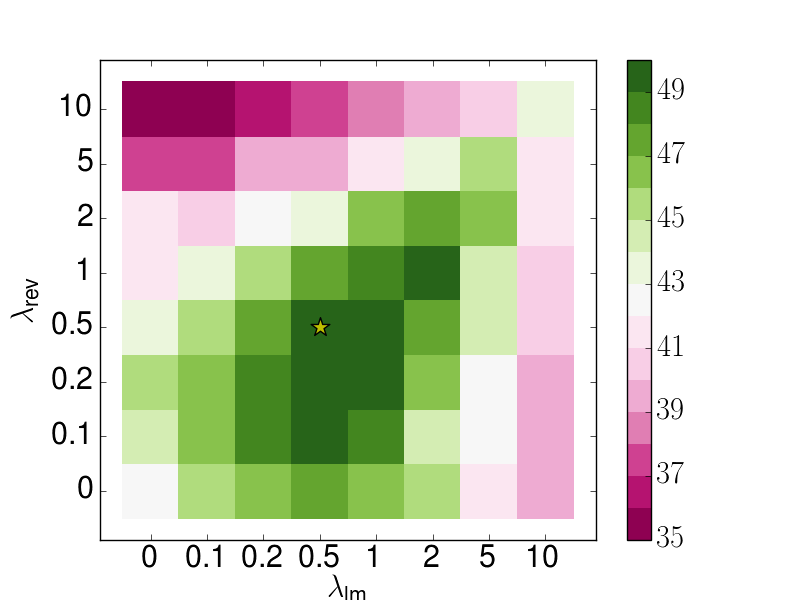
\includegraphics[scale=0.36]{0.png} & 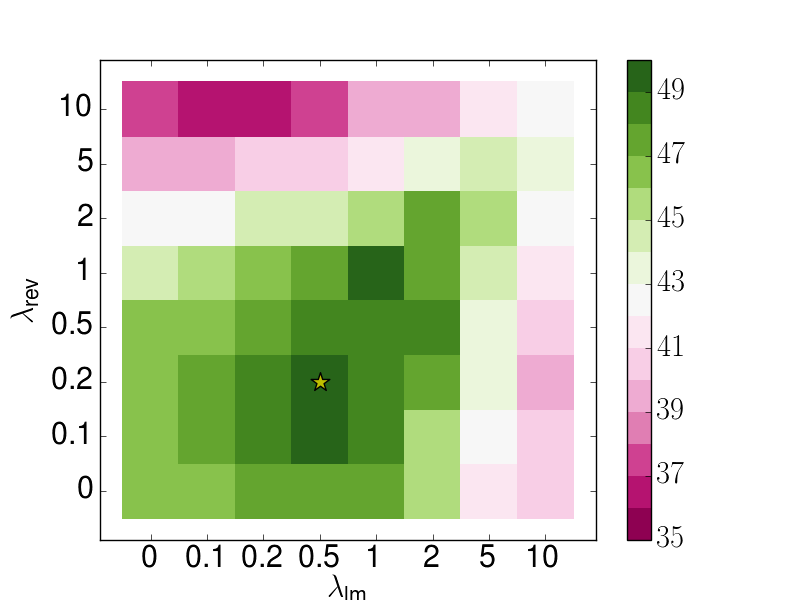
\includegraphics[scale=0.36]{1.png} \\
$\lambda_\text{fwd} = 0.1$ & $\lambda_\text{fwd} = 2$ \\
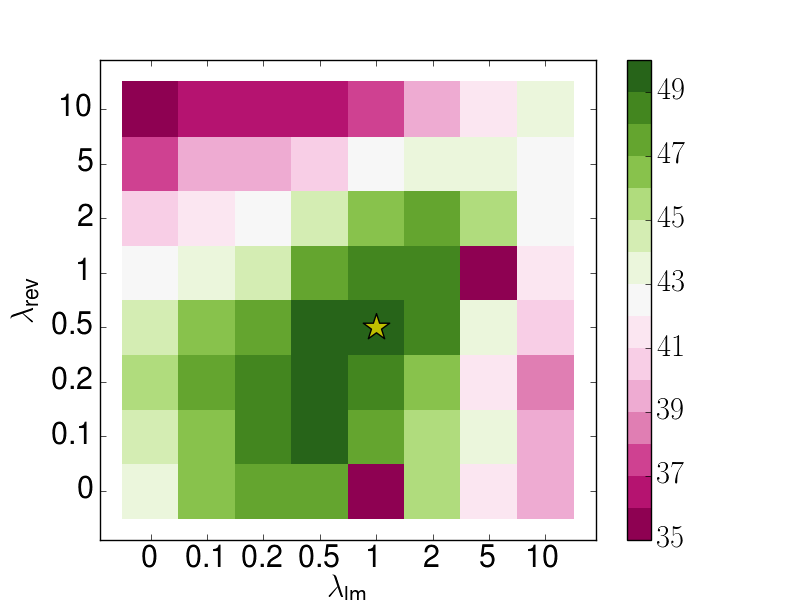
\includegraphics[scale=0.36]{0_1.png} & 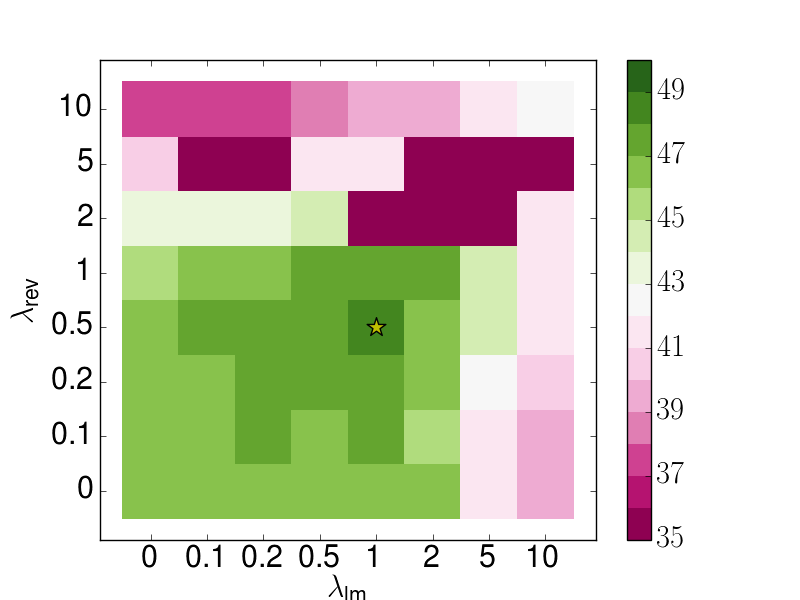
\includegraphics[scale=0.36]{2.png} \\
$\lambda_\text{fwd} = 0.2$ & $\lambda_\text{fwd} = 5$ \\
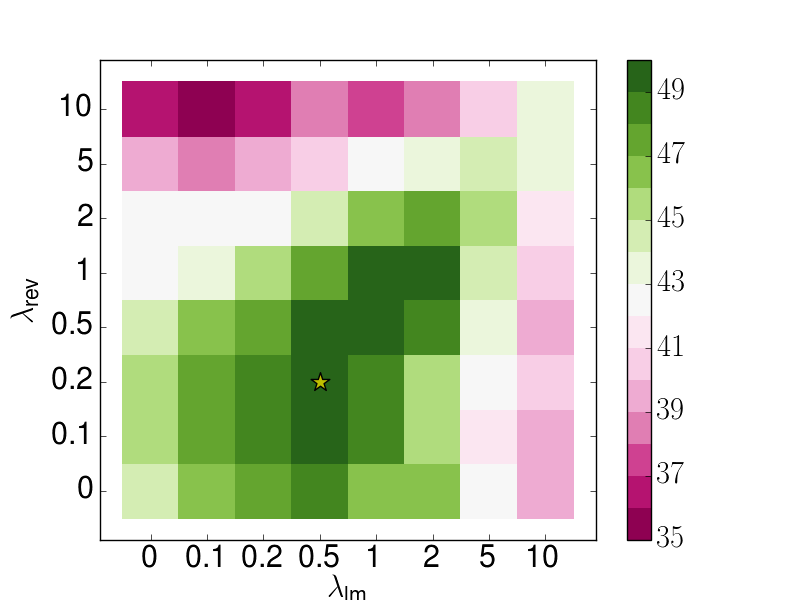
\includegraphics[scale=0.36]{0_2.png} & 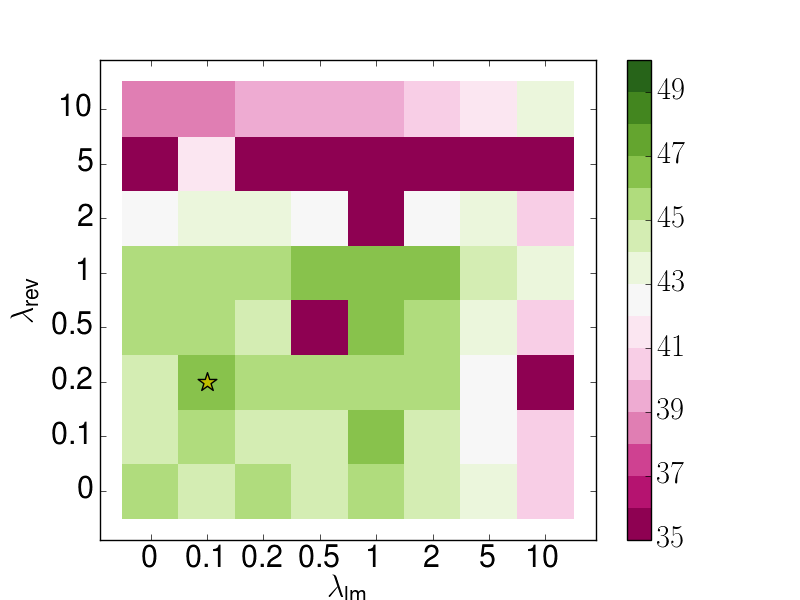
\includegraphics[scale=0.36]{5.png} \\
$\lambda_\text{fwd} = 0.5$ & $\lambda_\text{fwd} = 10$ \\
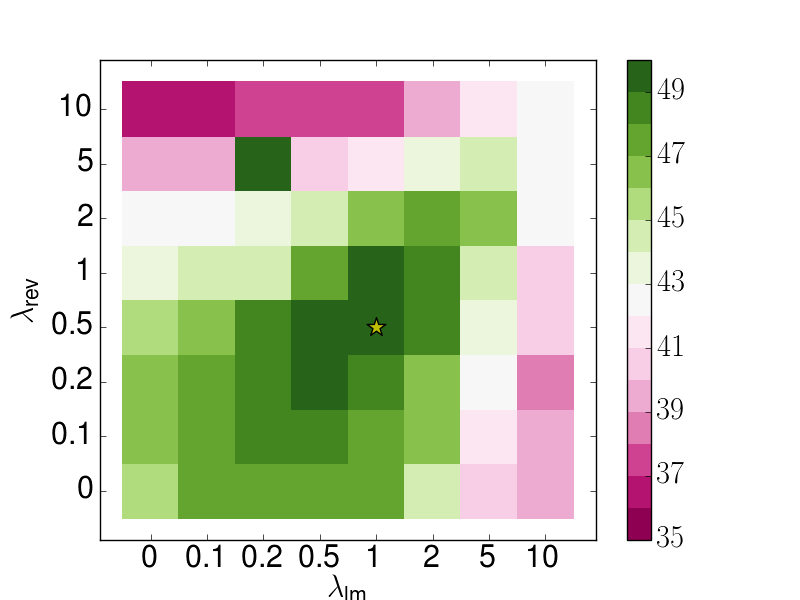
\includegraphics[scale=0.36]{0_5.png} & 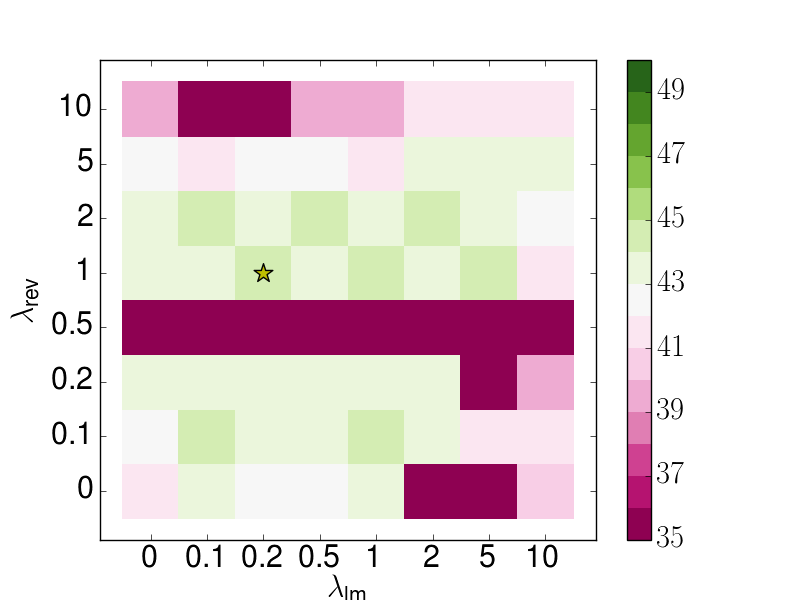
\includegraphics[scale=0.36]{10.png} \\
\end{tabular}
\caption{Plots of our grid search over $\lambda$s on BTEC. In each plot the best set of values is marked by a gold star.
The global optimum, $\lambda_\text{fwd}=0.1$, $\lambda_\text{rev}=0.5$, $\lambda_\text{lm}=1.0$ is marked with a larger gold star.}
\label{fig:grid_search}
\end{figure*}

The results of our grid search over $\lambda$s (using $c_\text{puct}=20$ and
200 rollouts) are visualized in Figure~\ref{fig:grid_search}.

We search over $\lambda_{\text{fwd}}$, $\lambda_{\text{rev}}$, and
$\lambda_{\text{lm}} \in \{0, 0.1, 0.2, 0.5, 1, 2, 5, 10\}$ and find the
optimal values to be $\lambda_\text{fwd}=0.1$, $\lambda_\text{rev}=0.5$, and
$\lambda_\text{lm}=1.0$, with a BLEU score of 50.57.

\begin{table}
\centering
\begin{tabular}{r l l}
\toprule
Rollouts & BLEU & Loss \\
\midrule
1 & 32.03 & 1.17 \\
2 & 36.77 & 0.86 \\
5 & 42.32 & 0.65 \\
10 & 43.94 & 0.56 \\
20 & 44.97 & 0.50 \\
50 & 45.83 & 0.46 \\
100 & 46.06 & 0.44 \\
200 & 46.61 & 0.42 \\
500 & 46.68 & 0.41 \\
1000 & \textbf{46.75} & \textbf{0.40} \\
\bottomrule
\end{tabular}
\caption{Results with full Monte Carlo sampling on our dev sets.}
\label{tab:monte_carlo}
\end{table}

\begin{table}
\centering
\begin{tabular}{r l l}
\toprule
$k$ & BLEU & Loss \\
\midrule
1 & 42.69 & 3.93 \\
2 & 46.12 & 3.67 \\
5 & \textbf{48.83} & 3.44 \\
10 & 48.71 & 3.32 \\
20 & 48.58 & 3.24 \\
50 & 48.30 & 3.16 \\
100 & 48.27 & 3.12 \\
200 & 47.12 & \textbf{3.08} \\
\bottomrule
\end{tabular}
\caption{Results of rescoring $k$ best lists using our reverse and language models}
\label{tab:rescoring}
\end{table}

\end{document}
